\documentclass{beamer}
\usetheme{CambridgeUS}
\usecolortheme{default}
\setbeamercolor{itemize item}{fg=darkred!80!black}

\makeatletter
\setbeamertemplate{footline}
{
  \leavevmode%
  \hbox{%
  \begin{beamercolorbox}[wd=.333333\paperwidth,ht=2.25ex,dp=1ex,center]{author in head/foot}%
    \usebeamerfont{author in head/foot}F. Massa, A. Fagiolini
  \end{beamercolorbox}%
  \begin{beamercolorbox}[wd=.333333\paperwidth,ht=2.25ex,dp=1ex,center]{title in head/foot}%
    \usebeamerfont{title in head/foot}Monitoring update
  \end{beamercolorbox}%
  \begin{beamercolorbox}[wd=.333333\paperwidth,ht=2.25ex,dp=1ex,right]{date in head/foot}%
    \usebeamerfont{date in head/foot} April, 24th 2017\hspace*{2em}
    \insertframenumber{} / \ref{Conclusions}\hspace*{2ex} 
  \end{beamercolorbox}}%
  \vskip0pt%
}
\makeatother

\setbeamercolor{section in head/foot}{fg=white, bg=darkred!95!white}

\setbeamercolor{palette quaternary}{use=structure, bg=darkred!80!black} % changed this


\setbeamertemplate{headline}{%
\leavevmode%
  \hbox{%
    \begin{beamercolorbox}[wd=\paperwidth,ht=2.5ex,dp=1.125ex]{palette quaternary}%
    \insertsectionnavigationhorizontal{\paperwidth}{}{\hfill \hfill}
    \end{beamercolorbox}%
  }
}

\title{Highway simulator: \\
Monitoring update}
%\subtitle{Laurea Magistrale in Fisica}
%\author{Federico Massa}
%\institute{\large{Laurea Magistrale in Fisica \\
%Universit\`a di Pisa}}
\date{\small April, 24th 2017}

%\setbeameroption{show notes}
\setbeameroption{hide notes}
\setbeamertemplate{navigation symbols}{}

\usepackage{tikz}
\usetikzlibrary{decorations.pathreplacing}
\usetikzlibrary{positioning, calc}
\newcommand{\tikzmark}[1]{\tikz[overlay,remember picture] \node (#1) {};}

\usepackage{amsmath}% mathtools includes this so this is optional
\usepackage{mathtools}
\usepackage[export]{adjustbox}
\usepackage{multimedia}
\usepackage{multirow}
\usepackage[utf8x]{inputenc}
\usepackage{enumerate}
\usepackage{tcolorbox}
\definecolor{dred}{RGB}{200, 0, 0}

\begin{document}

%-----------------------------------------

{\setbeamertemplate{footline}{}
\setbeamertemplate{headline}{}
\begin{frame}
\titlepage
\bigskip
\medskip
\centering\small Federico Massa, Adriano Fagiolini
\end{frame}}
\addtocounter{framenumber}{-1}

\section{Introduction}
\begin{frame}
\frametitle{Why we needed an update}
\textbf{What we were doing}
\begin{itemize}
	\item We were trying to monitor the behaviour of a vehicle
		  with a discrete states automaton running different
		  controllers.
 	\item The recognition of the discrete state was made via 
 		  a forward prediction of the vehicle's continuous state,
 		  that was compared with the controller model that we
 		  supposed to know (first mayor problem)
  	\item The monitoring itself was achieved by evaluating the
  		  rules (that we also supposed to know from the constructor, second 
  		  mayor problem) that determined the transition between
  		  discrete states. Uncertain cases were due to the 
  		  partial vision of the observer with respect to the 
  		  monitored vehicle's surroundings.
\end{itemize}
\end{frame}

\begin{frame}
\frametitle{Why we needed an update}
\textbf{What we do now}
\begin{itemize}
	\item We monitor the behaviour of a vehicle based on the
		  abstract features of its movements. This way, we can
		  monitor a vehicle regardless of the dynamic model 
		  (it could also be manually-driven)
 	\item Instead of the recognition of the discrete state,
 		  we try to recognize the abstract \textbf{action} 
 		  that the vehicle is pursuing. 
  	\item The monitoring is now based on the definition
  		  of some basic \textbf{social rules}, that 
  		  are defined in an abstract way as the list of
  		  conditions that make a certain action forbidden.
\end{itemize}

To achieve this, we only need:
\begin{itemize}
\item The sensor data of all the vehicles visible to the observer (x, y 
      on the highway plane, at least) + some kind of vehicle ID to 
      follow its trajectory.
\item A list of possible actions that the monitored vehicle can do.
\item The implementation of the social rules that are being monitored.
\end{itemize}
\end{frame}

\begin{frame}
\frametitle{Configuration}

In the configuration file it is possible to choose, for every vehicle in the environment:
\begin{itemize}
\item Initial continuous and discrete state;
\item Geometrical parameters (Type of vehicle);
\item Dynamic model (Physical Layer type);
\item Automaton type;
\item Sensor errors.
\end{itemize}


\bigskip
\bigskip
\bigskip

The action recognition and rule monitor systems are very general and should work in any realistic case (if correctly tuned...see later on).

\end{frame}

\section{Action recognition}


\begin{frame}
\frametitle{First step: the action recognition}
An action is abstractly defined as a vehicle behaviour. Examples of
it include 
\begin{itemize}
\item \textit{left/right lane change}
\item \textit{overtake}
\item \textit{brake}
\item ...
\end{itemize}

We could also imagine a more sophisticated action recognition system
to include nuances of these basic actions, like \textit{slow left lane change} or
\textit{abrupt left lane change}.\\

\textbf{What the observer need to know:}

The observer vehicle should have a list of possible actions that the 
monitored vehicle can do. The action recognition system is now \emph{independent} from the monitored vehicle's model. 
\end{frame}

\begin{frame}
\frametitle{How the action recognition works}
In order to recognize an action, the observer needs to:
\begin{itemize}
\item Identify the monitored vehicle;
\item Keep track of the visible vehicles' sensor data for a finite interval of time.
\end{itemize}

Each action is recognized independently $\rightarrow$ concurrent actions are possible.

\bigskip

An \textbf{Action Manager} continuously listens to each action and verifies if the trajectory of the monitored vehicle is compatible with that action. If it is, the action is successfully recognized.

\end{frame}

\begin{frame}
\frametitle{The Action Manager structure}
Specific actions (LeftAction, RightAction...) inherit from abstract class Action. The ActionManager initializes several \textit{listeners}, i.e. actions that the system can recognize.
\bigskip
\bigskip
\bigskip

\centering
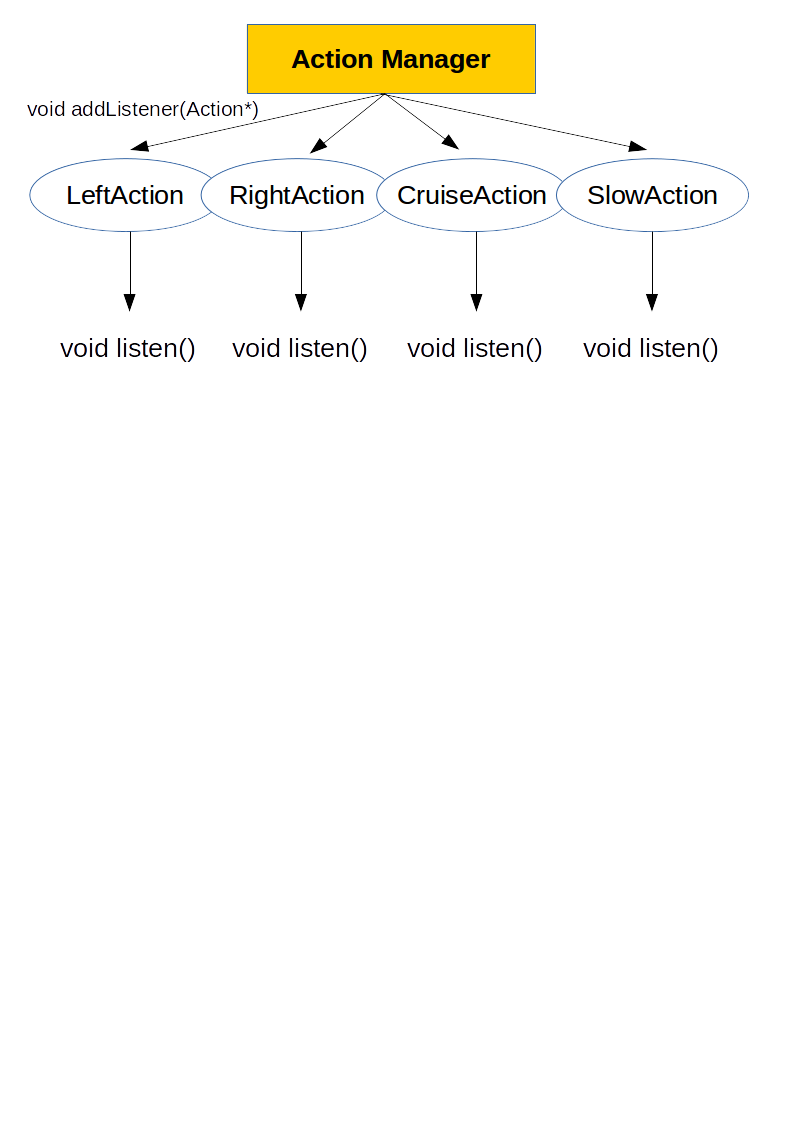
\includegraphics[scale=0.5]{ActionManager}

\end{frame}

\begin{frame}
\frametitle{listen() cycle}
If an action is registered in the ActionManager listener list, it enters a cycle:\\

\centering
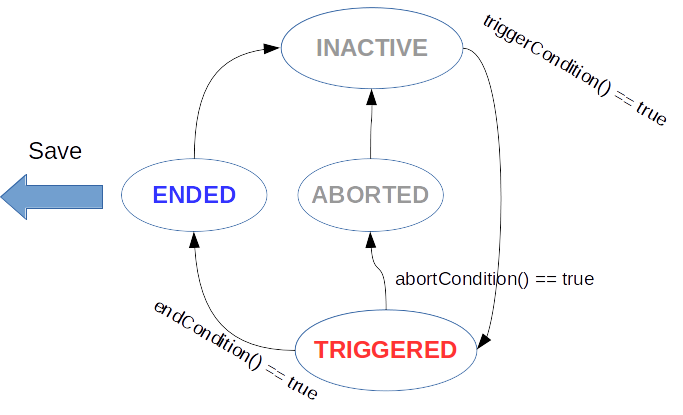
\includegraphics[scale=0.6]{ListeningCycle2}

\end{frame}

\begin{frame}
\frametitle{LeftAction example}

We use the following parameters (also using the N-points trajectory):
\begin{itemize}
\item $\Delta y$: Transversal distance covered in the recorded trajectory (last y - initial y);
\item $\mu_y$: Average transversal position;
\item $\sigma_y$: Standard deviation of transversal position.
\item f: constant between 0 and 1 (needs tuning);
\item $\Delta y_{tolerance}$: transversal position tolerance on central position (needs tuning);
\item $\epsilon_y$: transverse position sensor error. 
\end{itemize}

\bigskip

\begin{description}
\item[triggerCondition()] 
$ \Delta y > f\cdot v_{max}$ \\
 $\ \ \ \ \ \ \ |y_{init} - y_{initLane}| < \Delta y_{tolerance} + 3\cdot\epsilon_y$

\item[endCondition()] 
$\ \ \ \ |\mu_y - y_{targetLane}| < \Delta y_{tolerance} + 3\cdot\epsilon_y/\sqrt{N}$ \\
$\ \ \ \ \ \ \ \ \sigma_y < \epsilon_y$

\item[abortCondition()] \ \ After trigger time, the vehicle has disappeared.
 
\end{description}
\end{frame}

\begin{frame}
\frametitle{LeftAction video}

\movie[externalviewer]{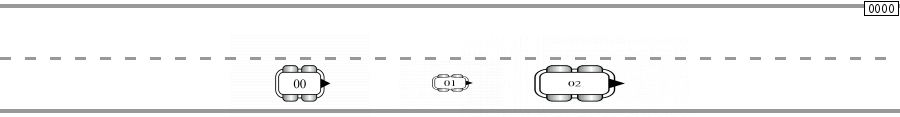
\includegraphics[scale=0.5]{leftActionVideo.png}}{leftActionVideo.avi}

\end{frame}

\begin{frame}
\frametitle{Complete action example}

\movie[externalviewer]{\includegraphics<1>[scale=0.5]{ActionExample/F00000.png}}{ActionExample/actionVideo.avi}
\includegraphics<2>[scale=0.5]{ActionExample/F00007.png}
\includegraphics<3>[scale=0.5]{ActionExample/F00030.png}
\includegraphics<4>[scale=0.5]{ActionExample/F00040.png}
\includegraphics<5>[scale=0.5]{ActionExample/F00080.png}
\includegraphics<6>[scale=0.5]{ActionExample/F00125.png}
\includegraphics<7>[scale=0.5]{ActionExample/F00148.png}


\bigskip
\bigskip
\bigskip
\bigskip	

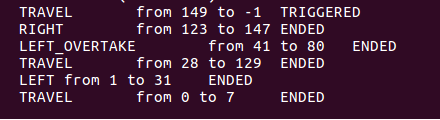
\includegraphics[scale=0.5]{Results}
\end{frame}

\section{Social rules monitoring}
\begin{frame}
\frametitle{Second step: implementation of social rules}
\begin{description}
\item[\textbf{\color{black}Observation:}] there are not unique correct behaviours, but there are {\color{dred}wrong} ones.
\end{description}

\onslide<2->
{
In practice, a set of social rules is composed by single rules with the
following features:
\begin{description}
\item[Category] A string useful to define groups of rules, such as "Safety rules", "Lane change rules", ...}
\item<3->[Event list] The rule is activated when at least one event is true.  Each event is composed by subevents and is activated when all subevents are true. Each subevent checks a specific logical condition on the monitored vehicle and its neighbors and can have a specific \textbf{area} of competence. \\
\item<4->[Evaluation mode] See after.
\end{description}
\end{frame}

\begin{frame}
\frametitle{Example: Italian-like highway rules}
\textbf{Safety rules}\\
\begin{itemize}
\item Safety distance, 1 event: ``Someone is in front of the monitored vehicle at less than x meters'';
\item Maximum speed, 1 event: ``The monitored vehicle is faster than x km/h''
\end{itemize}

\textbf{Left lane change rules}
\begin{itemize}
\item 1 event: ``Nobody is in front of the monitored vehicle'';
\item 1 event: ``Left lane is occupied'';
\item 1 event: ``The monitored vehicle is on the maximum lane''.
\end{itemize}

\textbf{Right lane change rules}
\begin{itemize}
\item 1 event: ``Right lane is occupied'';
\item 1 event: ``The monitored vehicle is on the minimum lane''.
\end{itemize}

\textbf{Travel rules}
\begin{itemize}
\item 1 event: ``Right lane is free'';
\end{itemize}

\textbf{Left overtake} allowed, \textbf{Right overtake} forbidden.

\end{frame}

\begin{frame}
\frametitle{Action Manager and Rule Monitor}
An object called \textbf{Rule Monitor} is used to check if the rules are 
violated, as the Action Manager ``listens'' to each action.\\

These two objects are independent, but they can communicate via the \textbf{rules categories}.\\

$\rightarrow$ Each action has a set of rule categories that it must follow. 

{Ex. LeftAction must follow the ``Safety'' rules and the ``Left Lane Change'' rules.}

\onslide<2->{
\begin{alertblock}{}This has several pros:\\
\begin{itemize}
\item Avoid the difficult abstraction task that links the specific action to the abstract rule it should follow;
\item Keeps the action and the rule systems well separated;
\item Different actions can share some rule categories.
\end{itemize}
}
\end{alertblock}

\onslide<3->{
$\rightarrow$ This also allow to make complex action managers without changing the rule system.}


\end{frame}

\begin{frame}
\frametitle{Action and rules}

\centering
\begin{tabular}{|c|c|} \hline
\textbf{Action} & \textbf{Rule categories} \\ \hline 
\multirow{2}{*}{LeftAction} & Safety \\ 
	& Left Lane Change \\ \hline
\multirow{2}{*}{RightAction} & Safety \\ 
	& Right Lane Change \\ \hline 
\multirow{2}{*}{TravelAction} & Safety \\ 
	& Cruise \\ \hline 
\multirow{2}{*}{LeftOvertakeAction} & Safety \\ 
	& Cruise \\ \hline 
\multirow{2}{*}{RightOvertakeAction} & Safety \\ 
	& Right Overtake \\ \hline 
\end{tabular}
\end{frame}

\begin{frame}

\frametitle{The Rule Monitor structure}
Just alike the Action Manager, the Rule Monitor object is used to initialize
the rule system and verify that the right rules are checked. At each instant:\\

\setbeamertemplate{enumerate items}[default]
\begin{enumerate}
\item<+-> Ask the Action Manager the list of triggered actions;\\ 
\item<+-> Extract the list of rule categories to be checked by merging the
	list of rule categories of each action;
\item<+-> For each rule category, take each rule and consider its ``Evaluation Mode'';
\item<+-> If the Evaluation Mode is on TRIGGER, the rule is checked only at trigger time. If it is on CONTINUOUS, the rule is checked every time until the action ends (e.g. Safety rules are generally in CONTINUOUS mode);
\item<+-> A rule is \textbf{true} if a wrong behaviour was spotted (at least one of the events is true), \textbf{uncertain} if the observer cannot tell 
if a rule is verified or not due to hidden areas (no events are true, at least one uncertain), \textbf{false} if the behaviour is correct  (all events are false).
\end{enumerate}
\end{frame}

\begin{frame}
\frametitle{LeftAction example}

Without sensor errors:\\
\movie[externalviewer]{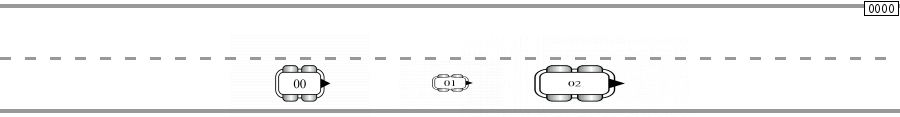
\includegraphics[scale=0.5]{leftActionVideo.png}}{monitorLeftActionVideoNoErrors.avi}

\bigskip
\bigskip

With sensor errors:\\
\movie[externalviewer]{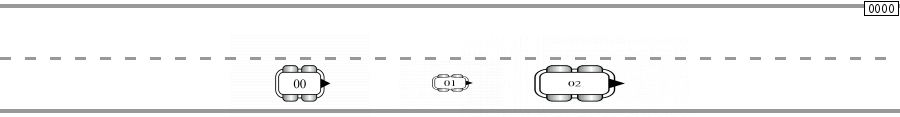
\includegraphics[scale=0.5]{leftActionVideo.png}}{monitorLeftActionVideoErrors.avi}

\end{frame}

\begin{frame}
\frametitle{Remarks on the C++ code}
The C++ code is mostly written using polymorphism, so that it is
very easy to make a more complex system without having to understand the
underlying code:\\

\begin{itemize}
\item Specific actions inherit from the Action class. To add a new action,
	it is only necessary to manually write the trigger, end and abort 			    conditions.
\item Specific set of rules inherit from the SocialRules class. After   		    manually
	writing a new set of rules it is possible to change the monitored rules
	by changing a single line of code.
\end{itemize}

A similar concept applies when wanting to change the vehicle geometry, dynamics or automaton. The code is written keeping flexibility in high regard.


\end{frame}

\begin{frame}\label{Conclusions}
\frametitle{Summing up}
The simulator should now be able to:
\begin{itemize}
\item Recognize and record list of actions done by the monitored vehicles;
\item Verify, if possible, if the monitored vehicle is following the rules;
\item Do this no matter the vehicle size, dynamic model, state transition rules (could also be manually driven in theory).
\end{itemize}


\begin{alertblock}{Critical point:}
Action parameters tuning
\end{alertblock}

Further studies:
\begin{itemize}
\item Use of consensus to improve the observer dataset (both to reduce sensor errors and to reveal the content of the hidden areas);
\item Reputation system: how to deal with infractions?
\item Roomba?
\item Possible application in Roborace?
\item Besides highways? 
\end{itemize}


\end{frame}
\end{document}

